\chapter{Design}
To develop an interface that satisfies the design requirements in \autoref{sec:designRequirements} and the final problem statement of this project, described in \autoref{sec:FPS}, some considerations were made in regards to the actual design of both the physical prototype and the virtual environment. This chapter describes the final design of the product.

\section{Context and User development}
When we started think about potential designs that could be used, we initially wanted make a different design for a different target group. We thought that this problem of visualizing a plant or tree in a context that only existed mentally could be applied at a garden center. A garden center is a retailer of different garden things, and they want to provide a good service, and sell many trees. Customers might be more willing to buy if they had the opportunity to see how their purchase would appear in their own garden. We already started conducting interviews at a garden center in Hillerød. However, during the demo day we found that the setup process was extensive and time consuming, as the demo'ers had to set up a new garden from scratch every time. This would likely be true even in a final product. We found that the transition between how a garden appeared on the prototype, and how it looked in VR, often caused the demo'ers to lose their sense of position in the garden. Simply getting the HMD off and on again added to the time between reviewing the garden designs as well. The people who made best use of the prototype were teams where one person would be an "architect" and one person would experience the changes made by the architect. It was very difficult to be creative for just one person. Combining this with results from the garden center survey ,that garden center customers had difficulties actually remembering what plants they had in their garden, it might be impossible for people to reconstruct their actual garden\\

In response to these problems we pivoted to a different target group and a different context. From our interviews with garden architects we knew that they face similar problems in visualizing their designs for the customers. Garden architects often are called upon for big reworks, or to design for gardens in newly built houses with no plants in them at all. While the opportunity cost of spending five minutes in garden center just to see what a new tree would look like is quiet high, the cost of spending that same amount of time for a once in your life time thing is very low. This also avoids the problem of not being able to remember what is in your garden, because you will be in that garden with the architect. Also there will be a two person team, the architect can show their idea to the client, and quickly make adjustments based on their input, and client won't have to take of the HMD.\\
This is how we ended up with the final design idea. From here decisions had to be made as to how to actually implement the design, and how to make it possible.


\section{Design development}
The initial idea was for a camera to recognize colors, shapes, sizes, and symbols on a simple user created sketch of a garden. This seemed to be the ideal prototype as it would give the user a lot of freedom in the creative process. Sketching has some issues in terms of consistency. We wanted the structure to be simple, and the elements of the prototype to be controlled for consistent recognition. The use of tokens also known as fiducial markers were determined to be the best solution for achieving consistency. The physical surface and the tokens placed on it would act as the only way to manipulate the world. Using a physical interface makes the process of manipulating the virtual world much more approachable to those not familiar with VR. It also encourages creativity more so than a digital system would. In terms of tracking the tokens the original idea was to have a large table with a camera mounted above it. From the camera image processing could be used to identify the tokens. Quick visualizations of what the early prototype would have looked like can be seen in Figure \ref{fig:previz1} and \ref{fig:previz2}

\begin{multicols}{2}
	\begin{figure}[H]
		\centering
		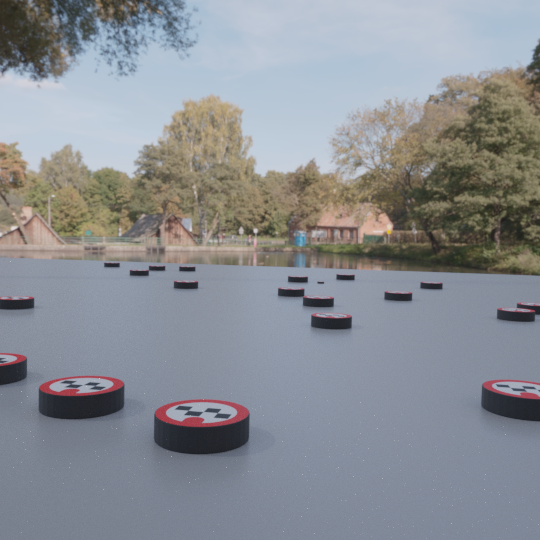
\includegraphics[width=1\linewidth]{figure/Design/closeup.png}
		\caption{Visualization of early design concept: close up of tokens}
		\label{fig:previz1}
	\end{figure}
	
	\begin{figure}[H]
		\centering
		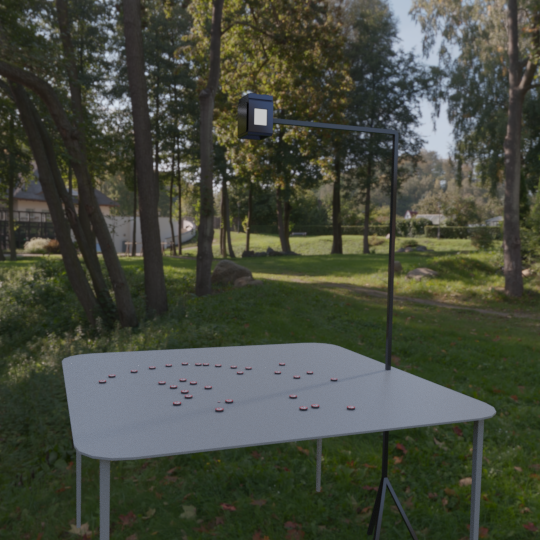
\includegraphics[width=1\linewidth]{figure/Design/sideview.png}
		\caption{Visualization of early design concept: table and camera}
		\label{fig:previz2}
	\end{figure}
\end{multicols}
A few changes were made to the original design though. We realized that users would likely be unable to recognize what a token was solely from pattern on top. This would be a huge issue with the product. One solution could be to make the tokens very distinct, for instance a pine tree and a an oak tree have very different silhouettes. Using silhouettes solves the human vision issue, but reduces the amount of tokens that the camera can recognize, because telling the difference between different varieties of the same species would be very difficult. So the garden architect would often be forced to place just a "pine" token rather than something specific like a European black pine.\\\\
To solve this issue we decided to separate the image processing from what the user saw. The camera would be moved beneath the table, and the table would be transparent. The top of the token would now display a 3D rendering of the plant it represented in VR, while the bottom now contained the marker used for object recognition. During the interviews some garden architects expressed concern regarding weight of the prototype. They work on the move, and would want to avoid something too heavy. In accordance the larger table was scraped in favor of a smaller box design. 

\section{The Physical Prototype}
The prototype consists of a lightweight box, of which four sides are laser cut MDF and the top is a square piece of acrylic. The bottom is open. A number of tokens may be moved around the surface of the box. The tokens are circular and 3D printed, with a colored marker on the bottom and a picture of the token's virtual counterpart on the top. A camera is placed at the bottom of box, looking up. 
The setup is connected to an HTC Vive with no modifications.

\subsection{The box}

The construction of the box consists of four identical sides measuring 570 by 300 by 300 mm. MDF (medium-density fibreboard) was chosen for the box as it is lightweight, sturdy, and easy to cut with a laser cutter. It is important that the prototype is lightweight as it must be transported to various locations for testing. The precise laser cutting of the sides means that the sides can be made with the interlocking parts that connect firmly without the need for mechanical locking parts. The main concern was ensuring the pieces form a tight fit.
\begin{figure}[H]
	\centering
	\includegraphics[width=0.5\linewidth]{figure/Design/boxVive.png}
	\caption{Shows the design of the box}
	\label{fig:boxVive}
\end{figure}
 Since material is removed during the laser cutting process, the design had to be purposely made too tight. The test cut worked well at first, but the fit became too loose after being put together and taken apart a few times. A tighter fit was then designed for the final cut of the prototype elements. To make sure that the box doesn't fall apart, the sides were glued together. 

The bottom of the box is left open for an easier setup.
The box is made to be tall enough that the camera can capture all of the acrylic surface in its field of view, which we determined was 570 mm.
%30,30,57 and 297
The top of acrylic is needed so that there is a place to put the tokens, which the camera can see.

The acrylic top of the box is a square, made to be fitted into the box, resting on wooden cubes glued to the sides of the box. The cubes are to be no more than a centimeter wide. Ideally finger joints would also be cut into the acrylic and the top of the sides of the box, allowing us to simply lock the top into place without the need for the wooden strips. This was however first thought of after the sides had been cut. Adding the additional cuts to the sides would be tricky to do with perfect accuracy, as even a slight error would ruin the fit. 
Holes are cut into the sides near the bottom to route cables for the webcam through, while doubling as carrying handles for easy transportation. 

\subsection{The tokens}

The physical construction of the tokens was not a cause of great concern. They simply needed to be circular, as most trees take up a circular amount of space. We chose 3D printing for the tokens because of consistency concerns, and for the ease of construction. The markers themselves are color prints on regular white printer paper, that are glued to the bottom of the tokens. Markers can be easily reprinted and replaced if a problem is found with the current image processing implementation. 
The size of the markers is made to be as small as possible while still working with the image processing aspect. It all depends on the quality of the webcam image. The worse quality the webcam delivers, the larger the markers need to be. With a proper DSLR camera we could scale down the markers considerably, but the software to make such a camera work as a webcam is expensive, and so for the prototype we went with a Logitech QuickCam® Communicate STX\footnote{Logitech QuickCam® Communicate STX product page: \url{http://support.logitech.com/en_us/product/quickcam-communicate-stx}}.\\

The marker is designed to have a thick stroke around its perimeter. This is what makes the program classify it as a marker. At one point, a line is drawn from the edge of the marker and slightly inwards. This lets the program determine the token's rotation vector. In the center of the marker, between 0 and 8 squares are placed.
\begin{figure}[H]
	\centering
	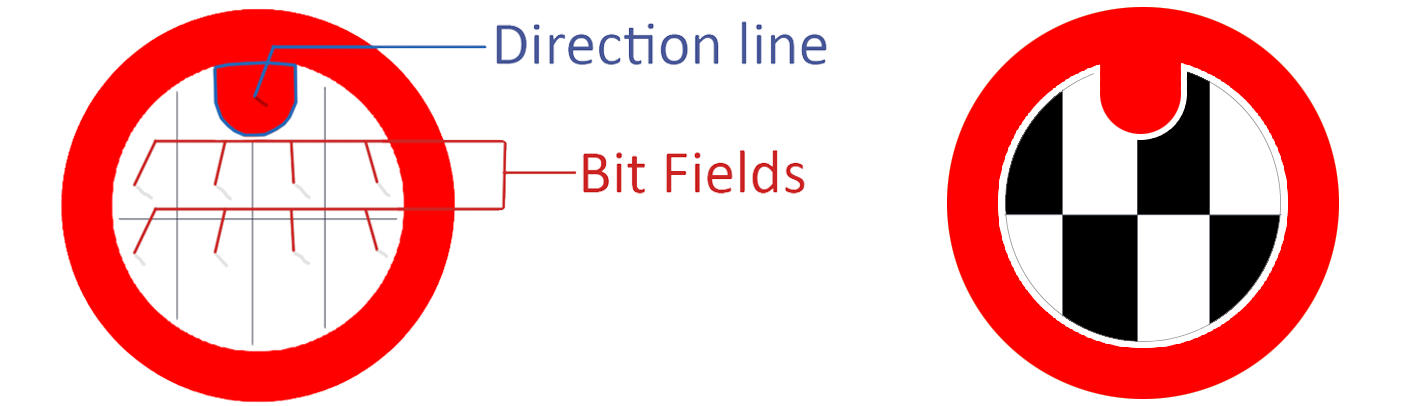
\includegraphics[width=1\linewidth]{figure/Design/markermap.png}
	\caption{Example marker indicating a value of 165}
	\label{fig:circle2}
\end{figure}

These each represent a bit, black indicating a 1 and white indicating a 0. They do not necessarily need to be square. The program looks at the center of each to get a brightness value.

\begin{figure}[H]
	\centering
	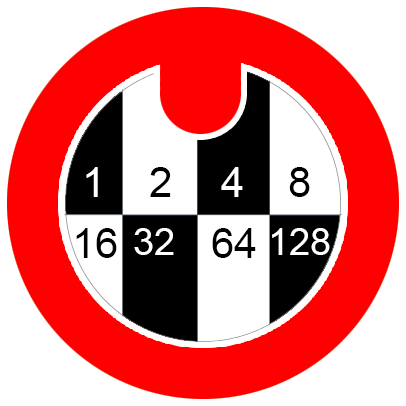
\includegraphics[width=0.3\linewidth]{figure/Design/markerValues.png}
	\caption{The value
		 each square represents}
	\label{fig:circle}
\end{figure}

This allows us to print a marker representing any one of 255 items. More could be added later, but for testing the prototype there is no need for more combinations as we are limited by the number of unique digital models.

A program was made to automatically generate markers as needed. It takes an array of integers and creates sheets of markers corresponding to the array. For the input \codeword{int[] markers = {1, 2, 4, 8, 16, 32, 64, 128, 100, 3, 9};} it returns the following image:

\begin{figure}[H]
	\centering
	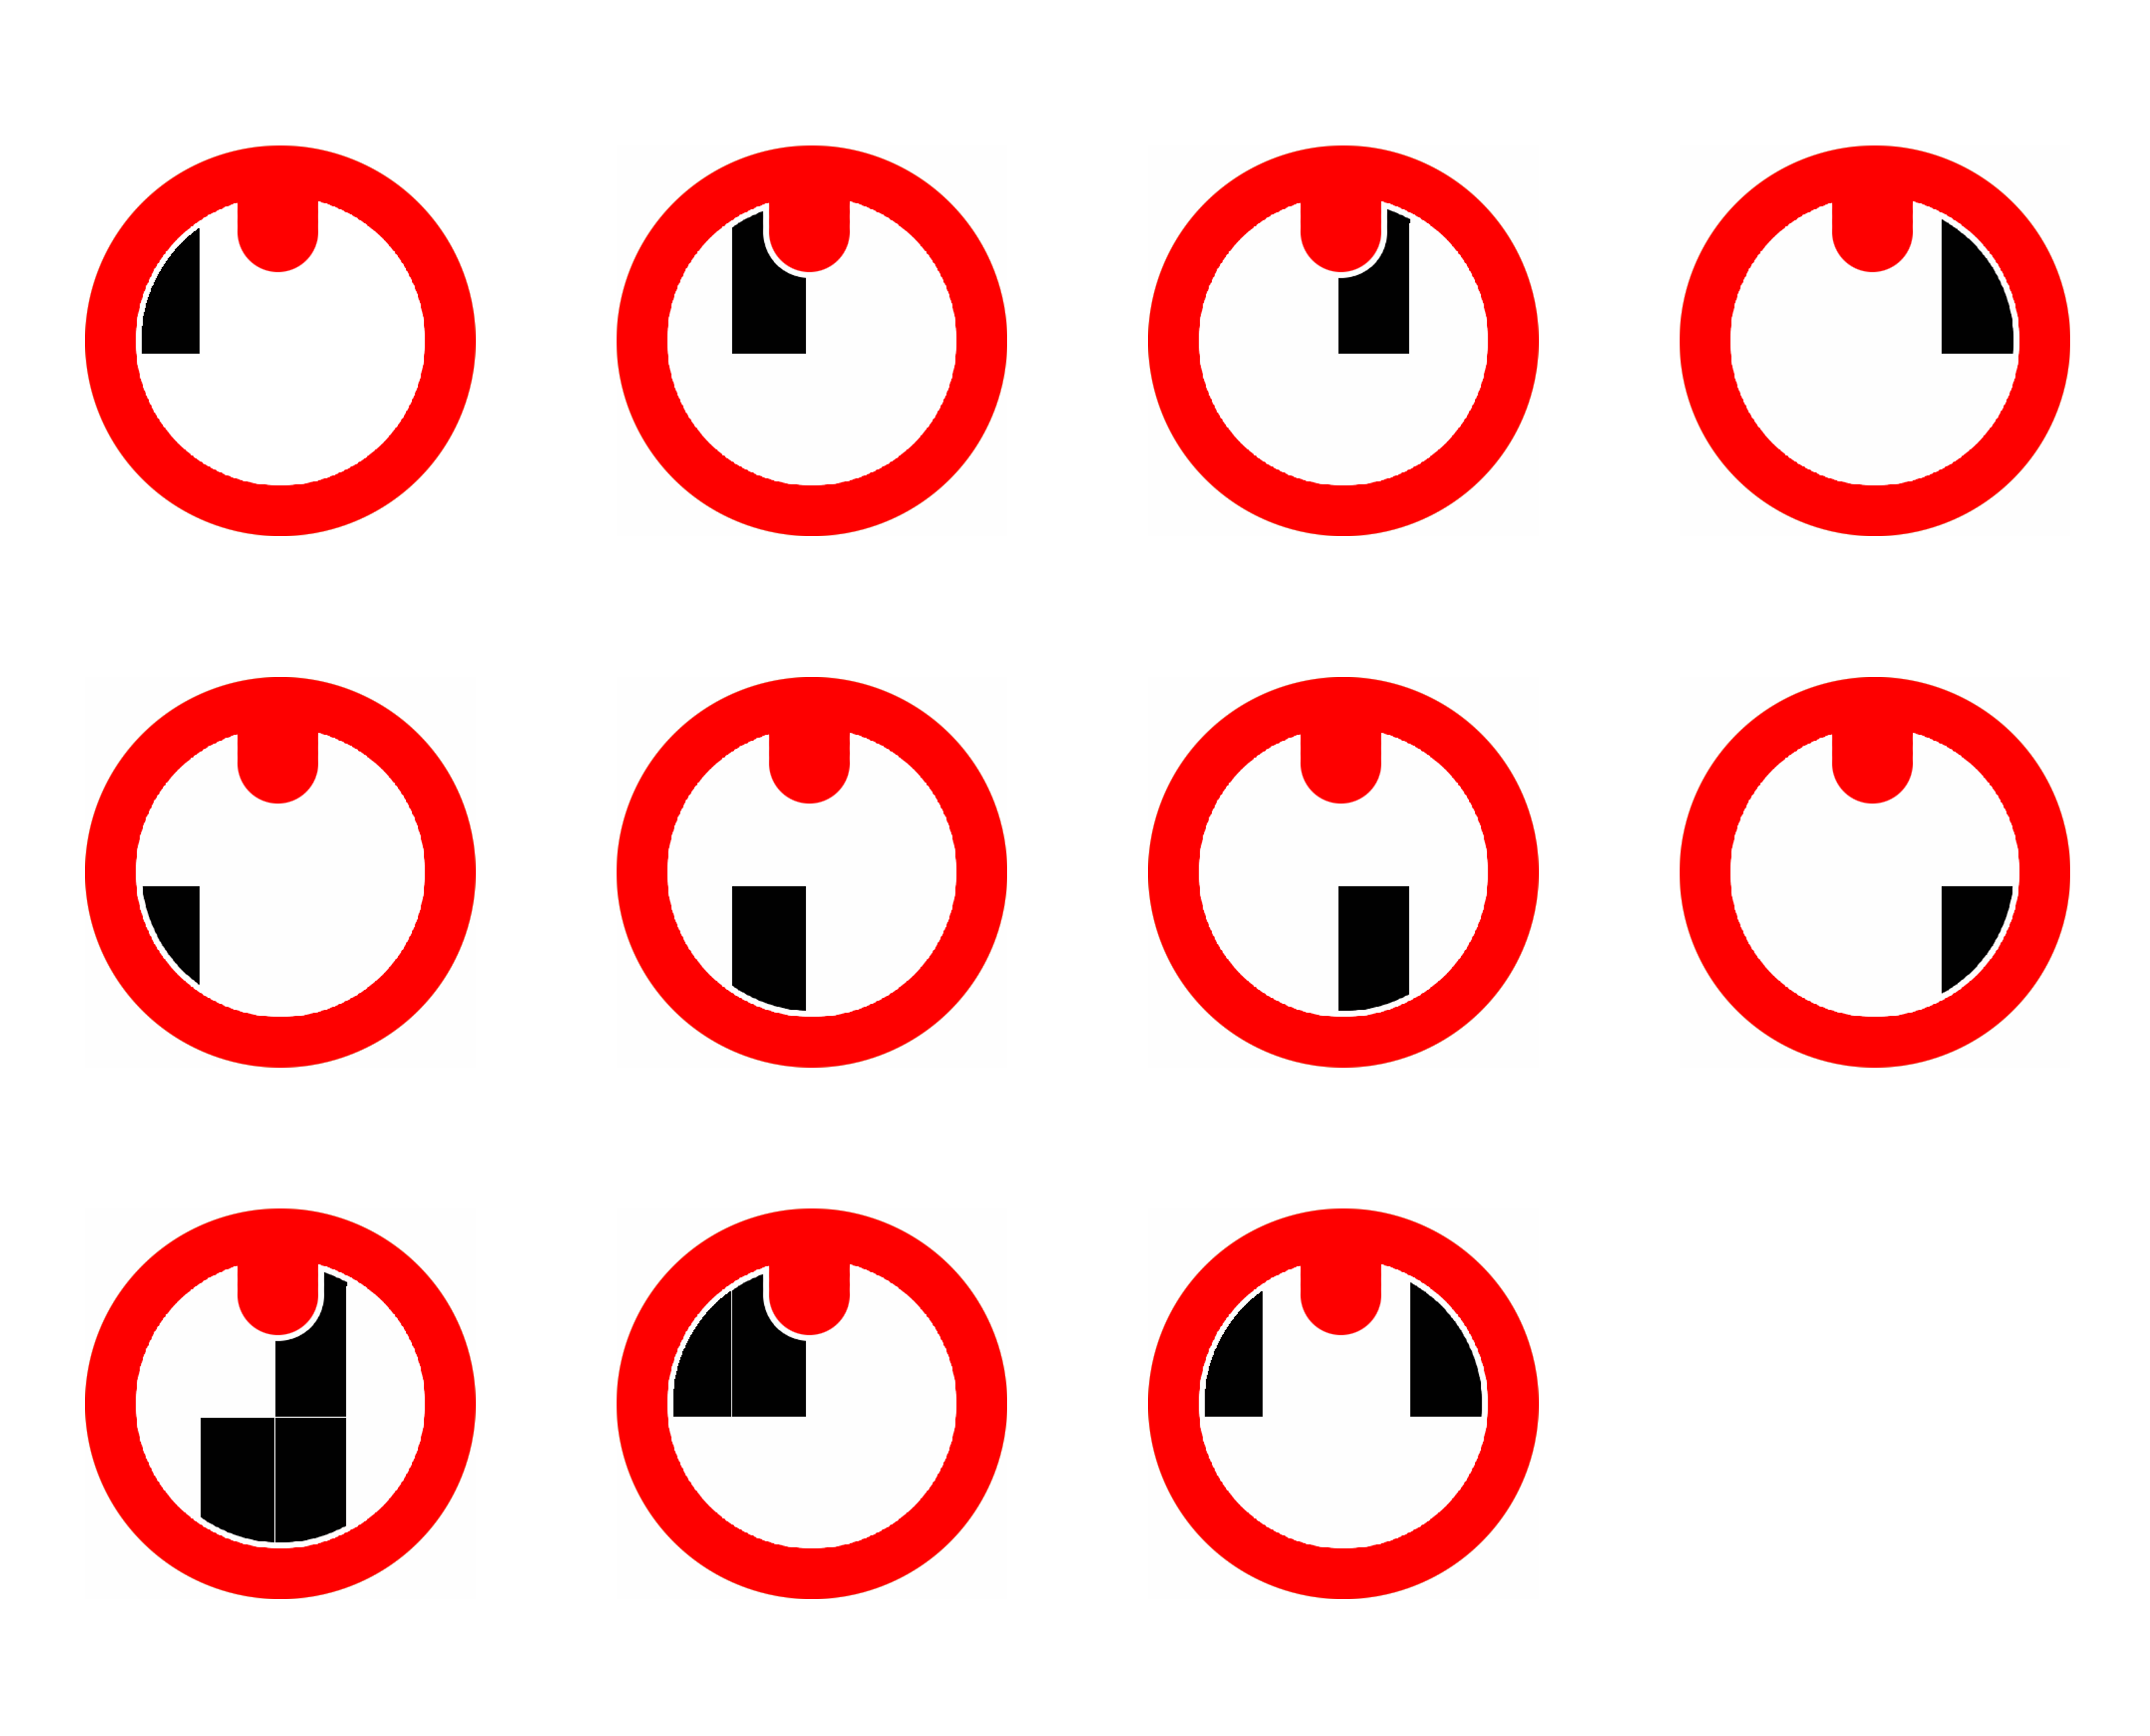
\includegraphics[width=0.7\linewidth]{figure/Analysis/result}
	\caption{Automatically generated markers}
	\label{fig:result}
\end{figure}


\section{The Virtual Environment}
The virtual environment was setup using Unity and the addition of the Steam VR SDK allowed us to connect the HTC Vive and place the user inside. All the 3D models were put into the Unity Assets. The technical details of this will be described in the Implementation chapter. This section describes the Virtual environment and the considerations that had to be made regarding the UI and the models.

\begin{figure}[H]
	\centering
	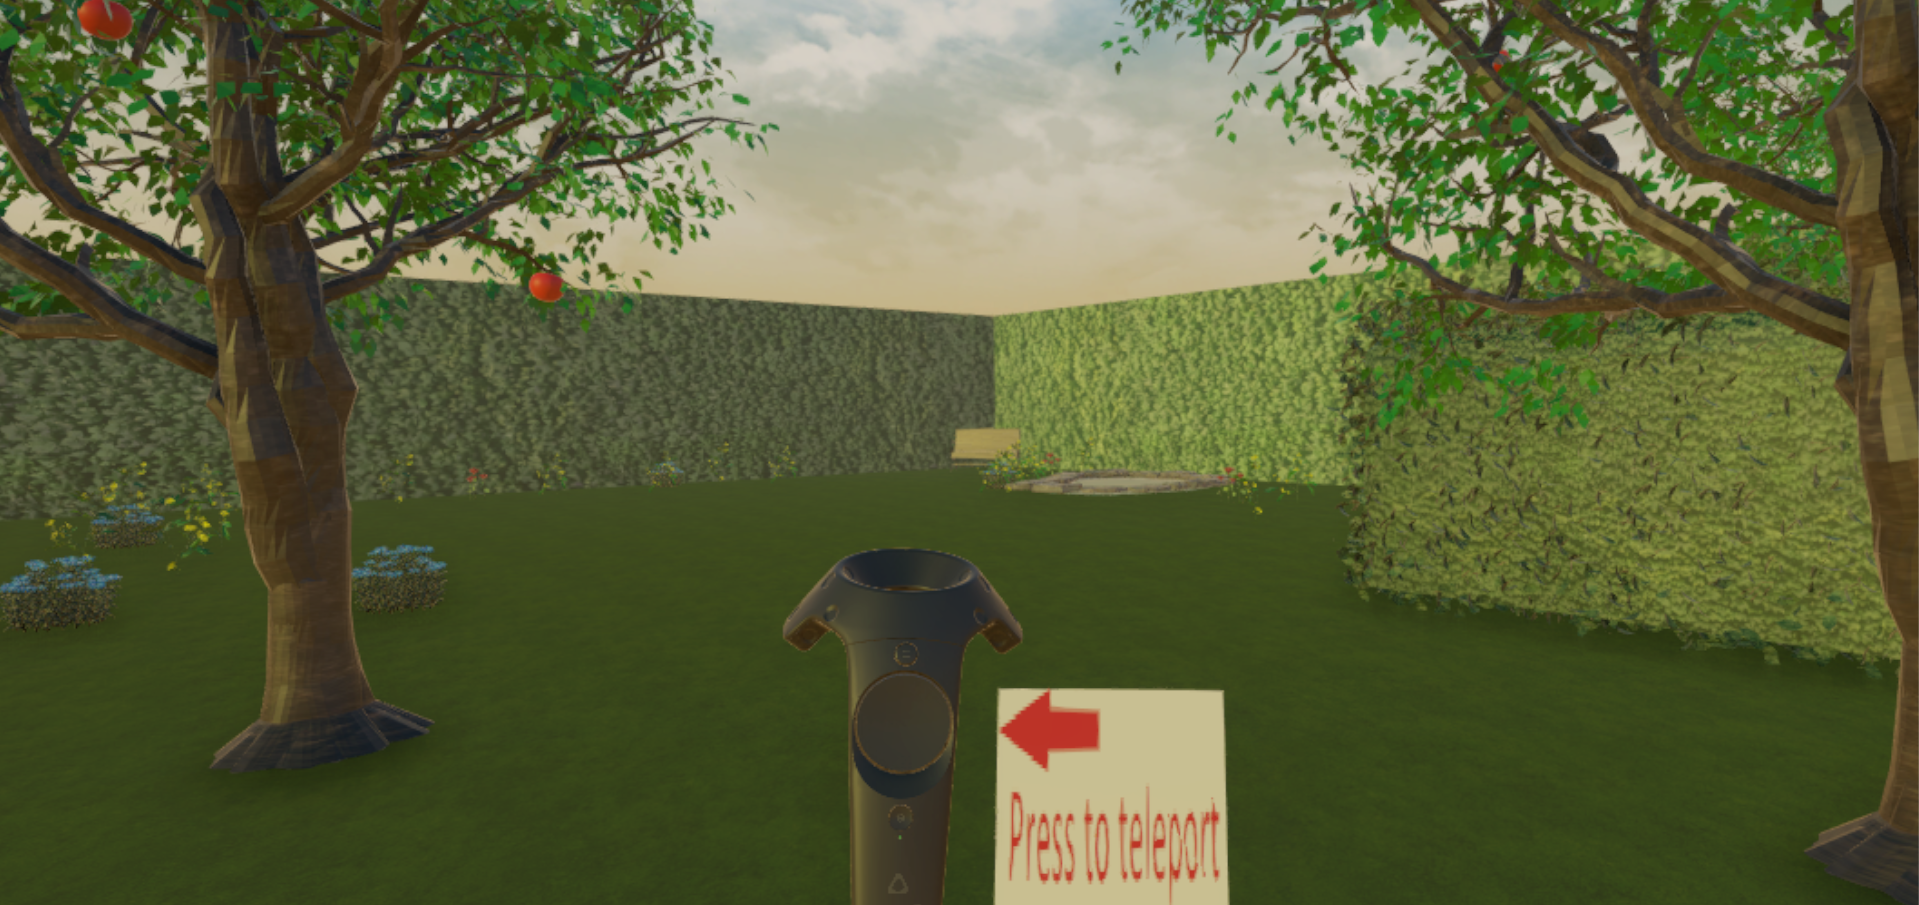
\includegraphics[width=0.9\linewidth]{figure/Design/vrPov.png}
	\caption{Image showing an example garden in the virtual environment from the point of view of the user wearing the VR headset.}
	\label{fig:vrPov}
\end{figure}


\subsection{The UI}
Not much is needed in terms of a user interface. All manipulation of the virtual objects is done by moving around the physical tokens. All the user can do inside the virtual world is move around. The VR controller is visible as a model which looks exactly like the physical controller, to minimize confusion. The only added element is a highlight of the trackpad with the text "Press to teleport" beside it (See \autoref{fig:vrPov}). This is added as there in an early test was a bit of confusion communicating which of the buttons allowed one to teleport around the environment.

\subsection{The models}
Inside the virtual environment there was a need for a lot of 3D models of different plants, trees, bushes etc. Objects that one would potentially use in designing a garden. We did not model these ourself, due to the limited timespan of this project. Instead we decided for this prototype to download free models, from the internet, as this allowed us to have a more diverse selection of objects for the architect to choose from during the designing process. This meant, however, that most of the objects listed in \autoref{sec:designRequirements}, were not added, as 3D models of these particular plants couldn't be found online. Roses, apple trees, lilacs and a few more objects were added from these sites: \url{https://free3d.com/} and \url{https://archive3d.net/}. A list of the object and their corresponding marker pattern can be seen below in \autoref{fig:markerOverview}

\begin{figure}[H]
	\centering
	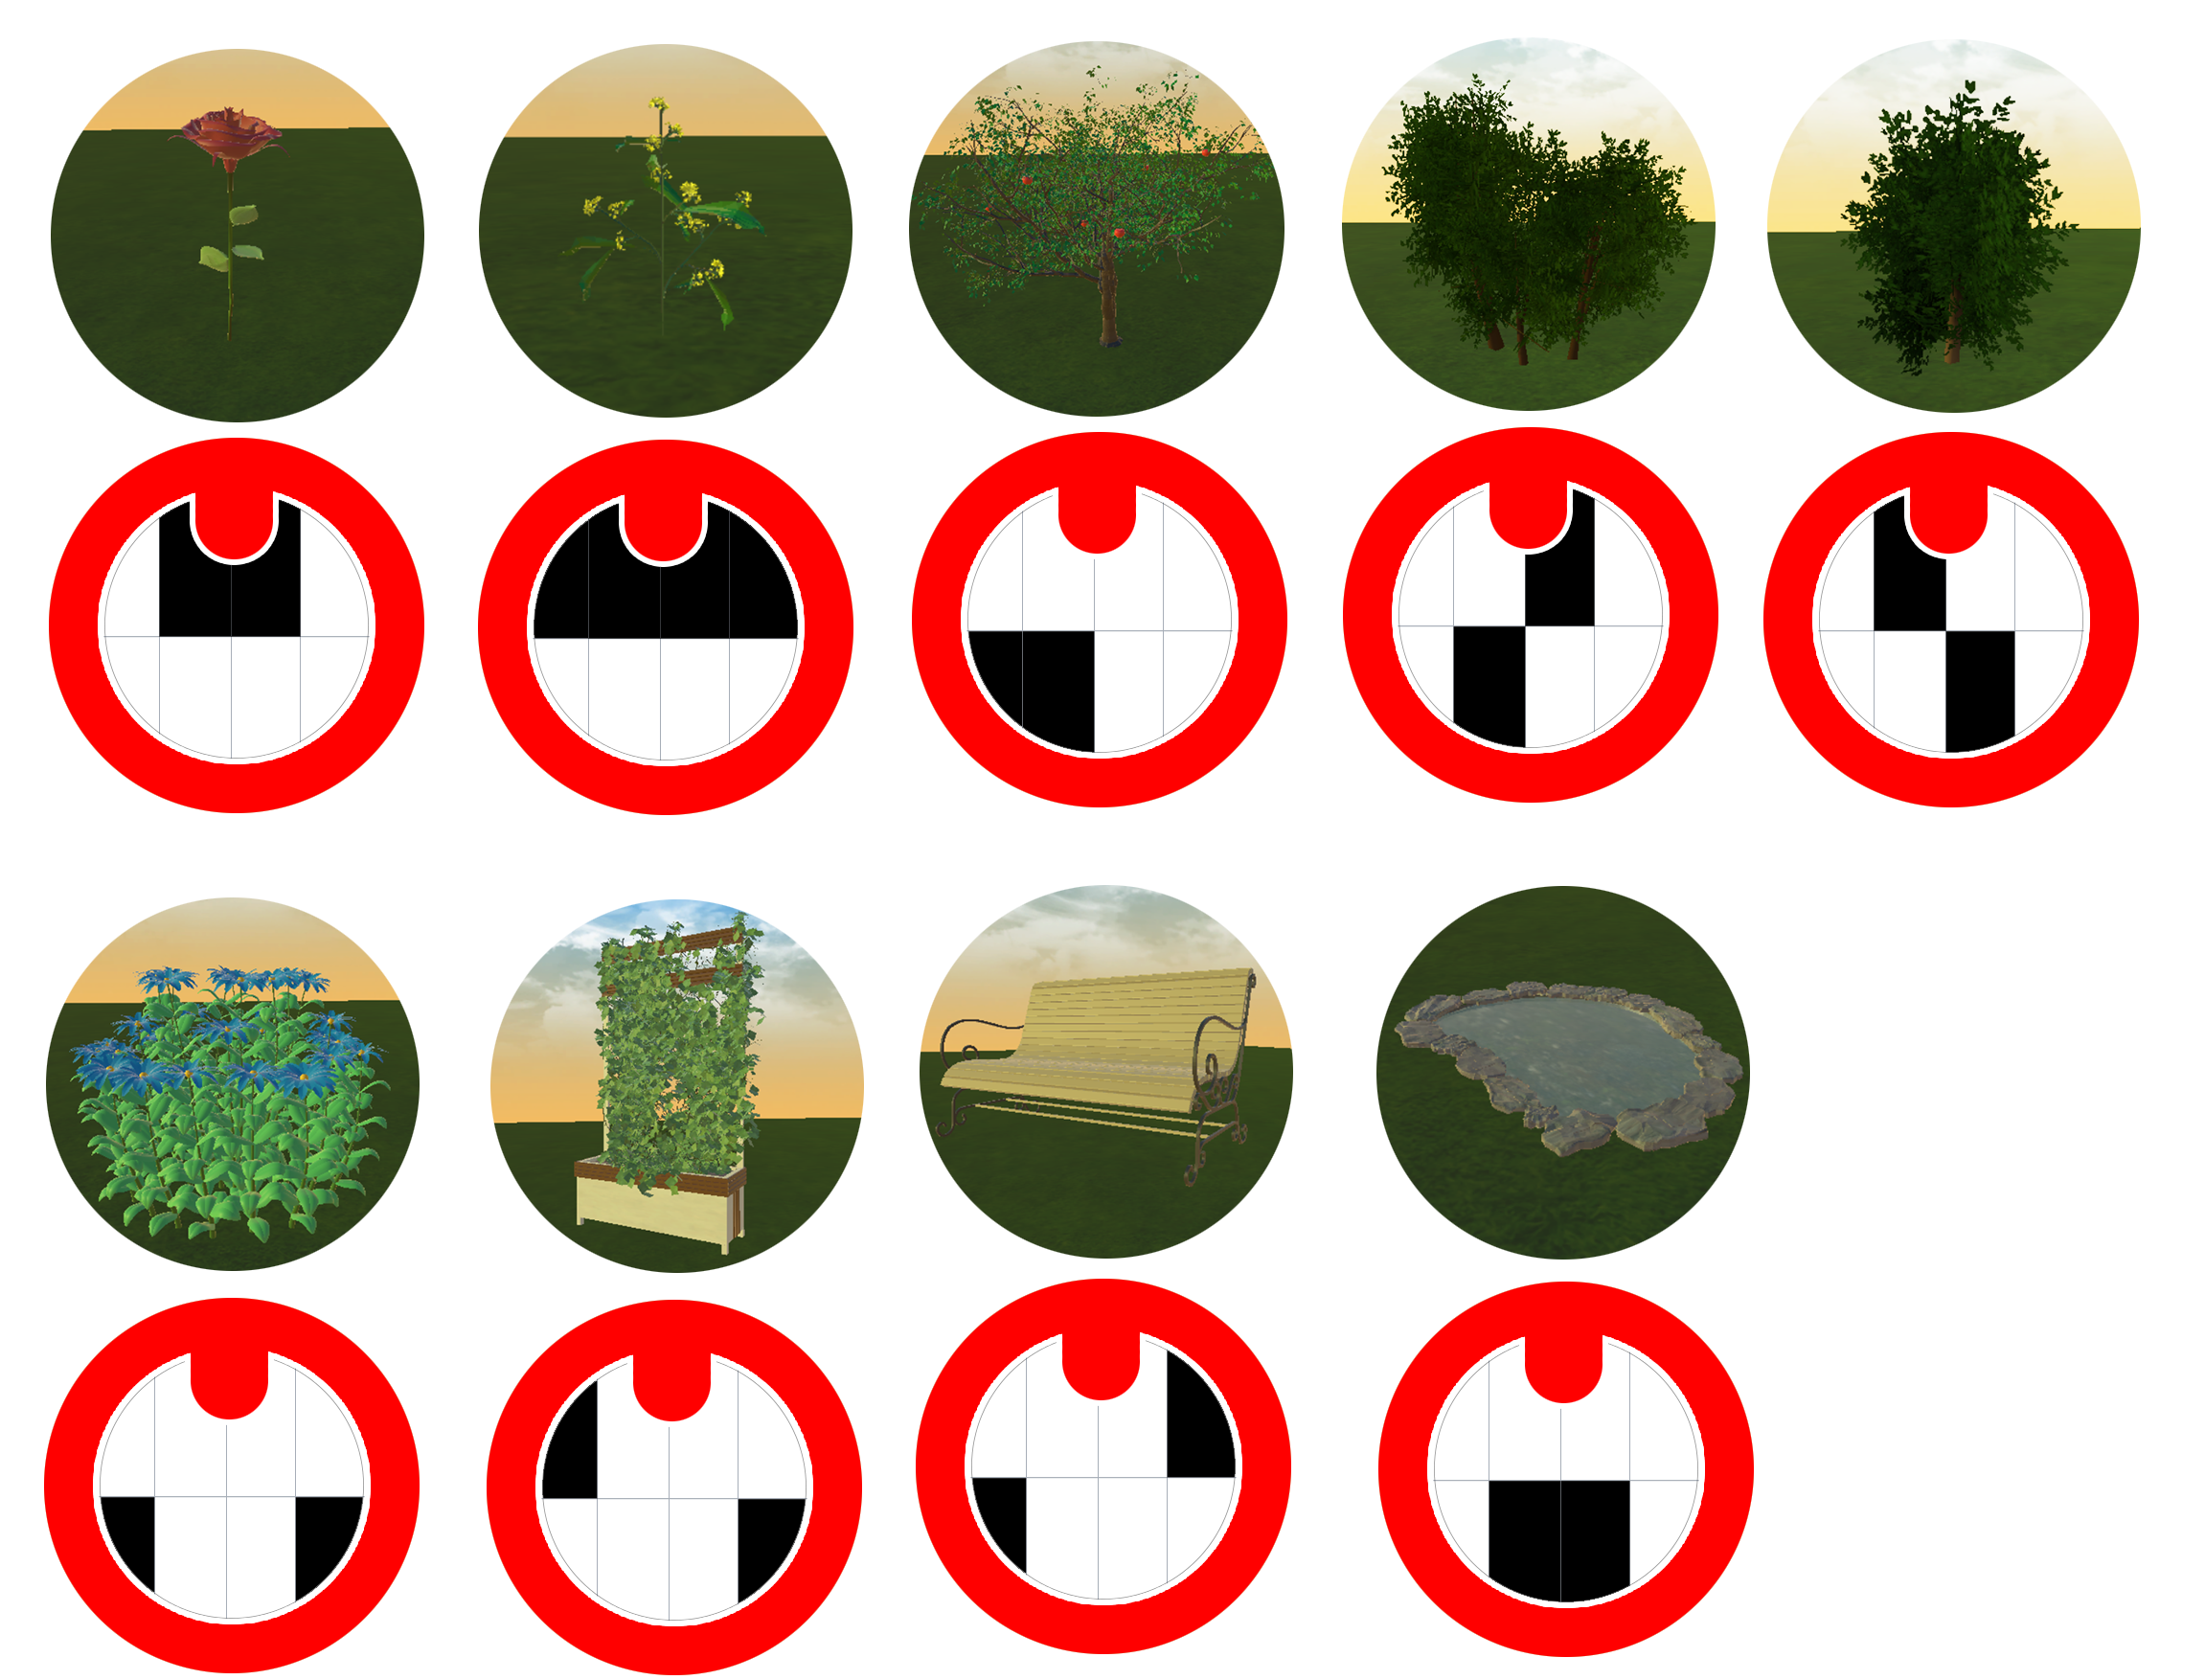
\includegraphics[width=0.9\linewidth]{figure/Appendices/markersOverview.png}
	\caption{List of objects that would appear within the 3D environment and the corresponding marker}
	\label{fig:markerOverview}
\end{figure}








